\label{chap:pt2_background}
This chapter provides the necessary background to introduce terms and concepts that may be unfamiliar to the reader, thereby facilitating the understanding of the work presented in this second part of the thesis.

\section{Physics Informed Machine Learning}

Informed Machine Learning (IML) refers to a learning paradigm in which learning is guided by a combination of data and prior knowledge. In this paradigm, the prior knowledge is provided by an independent source and explicitly incorporated into the machine learning pipeline~\cite{von2021informed}.

Physics-Informed Machine Learning (PIML) is a specific instance of this paradigm, in which machine learning models are trained to perform learning tasks while incorporating knowledge of the physical laws governing the phenomenon under study.

Prior physical knowledge can be incorporated into a neural network at different stages of the learning process, including the training data, the network architecture or model structure, and the learning algorithm~\cite{faroughi2024physics}. These different integration strategies result in different classes of physics-aware neural networks:

\begin{itemize}
	\item \textit{Physics-Guided Neural Networks} rely on training datasets generated from experiments or numerical simulations that already satisfy the underlying physical laws. In this case, physical knowledge is incorporated implicitly through the data used for training;
	
	\item \textit{Physics-Encoded Neural Networks} incorporate physical knowledge directly into the network architecture or model structure by designing its components and connections according to known physical laws;
	
	\item \textit{Physics-Informed Neural Networks} incorporate physical knowledge into the learning process through the loss function, where governing equations, boundary conditions, or conservation laws are included as additional terms.
\end{itemize}


\section{Forward problem and inverse problem}

In the scientific field, the difference between a forward problem and its inverse lies in the direction of the inference. In the former, the objective is to predict the distribution of observations given known distributions of the initial conditions and model parameters. In the latter, the objective is to infer the distributions of the initial conditions and model parameters from the available observations. Consequently, the inverse problem can be ill-posed when the available observations are insufficient to determine a unique solution.

As illustrated in Figure~\ref{fig:forward_inverse_problem}, in physics, the forward problem can be solved using numerical simulators since the physical laws governing the phenomenon under study are known. When, on the other hand, the inverse problem is considered, this information is not available, and only the observations can be used. Consequently, numerical simulators cannot be directly used to solve the inverse problem, and alternative strategies, such as neural networks, can be adopted.

\begin{figure}[hb]
	\centering
	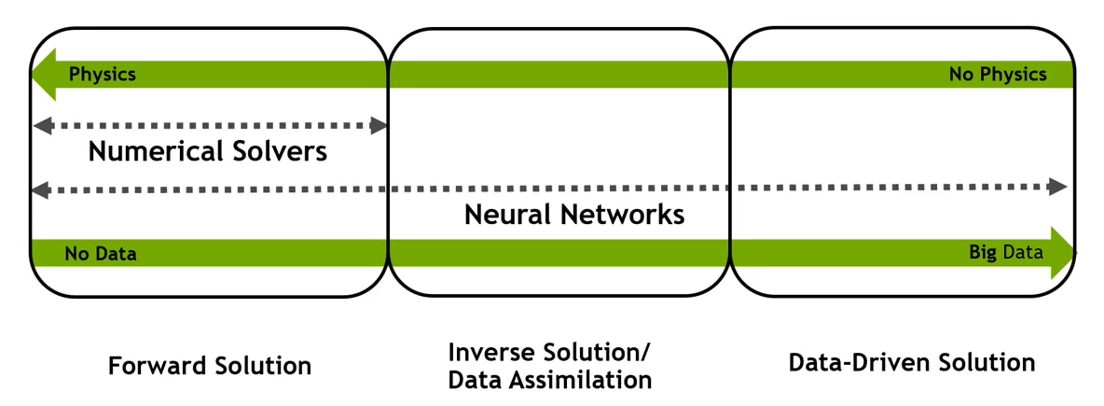
\includegraphics[width=0.8\linewidth]{figures/forward_inverse_problem.png}
	\caption{Solving forward problem and inverse problem}
	\label{fig:forward_inverse_problem}
\end{figure}

